\documentclass[11pt]{beamer}
\usepackage[utf8]{inputenc}
\usepackage[T1]{fontenc}
\usepackage{lmodern}
\usetheme{Boadilla}

\pgfdeclareimage[height=.8cm]{logo}{logo} 
\logo{\pgfuseimage{logo}}


	\author{Group 5  \\
	Emmanuel Owusu Ahenkan \\
    Volviane Saphir MFOGO \\
    Alex Sananka}
\title{Bootcamp Kaggle competition}
%\subtitle{}

%\logo{
\includegraphics[height=1.5cm]{logo.jpg}}


%	\logo{\begin{figure}[b]
%			\centering
%			
\includegraphics[width=0.7\linewidth]{logo}
%			\caption{}
%			\label{fig:logo}
%		\end{figure}
%	}
\institute{ African Masters in Machine Intelligence (AMMI- Ghana)\label{ammi}}
\date{\today, Accra}
%\subject{}
%\setbeamercovered{transparent}
%\setbeamertemplate{navigation symbols}{}

\AtBeginSection[]{
	\begin{frame}{Outline}
	\tableofcontents[currentsection]
\end{frame}
}

\begin{document}
	
	\maketitle
	\begin{frame}{Outlines}
		\tableofcontents
	\end{frame}
	
	\section{Introduction}
	

	
	\begin{frame}{Introduction}
			\frametitle{Introduction}
			\begin{itemize}
				\item Predicting the price of  wine based on a collection of  reviews and other product features. \\
				\item We use the Random Forest Regressor  and the XGBoost Algorithm to predict the prices of wine.
			\end{itemize}
					$\begin{array}{cc}
						\centering
						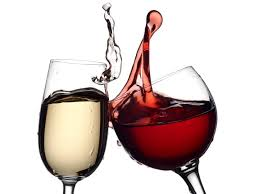
\includegraphics[width=0.35\linewidth]{wineImage}	& 
						\centering
						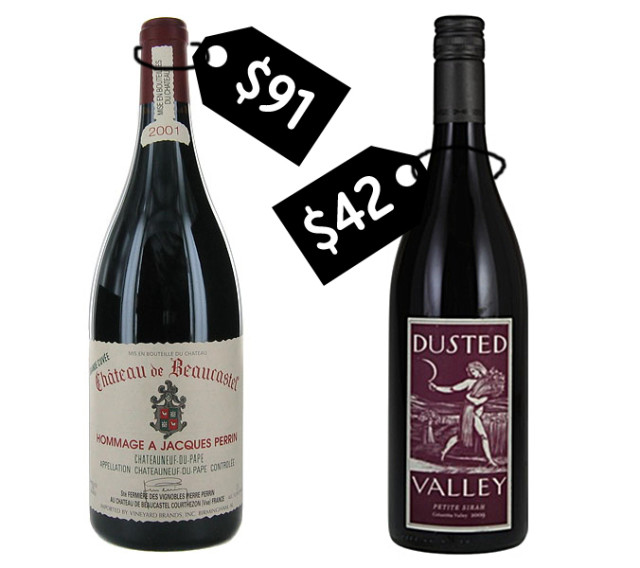
\includegraphics[width=0.35\linewidth]{Wine_Price_Illo_fva135} 
					\end{array}	$	
			
	\end{frame}
	
	
	\section{Explanatory Data Analysis}
	
	
		
	\begin{frame}{Explanatory Data Analysis}
	\frametitle{Explanatory Data Analysis}
	
	Let's start looking the information about our data. \\
	
	\centering
	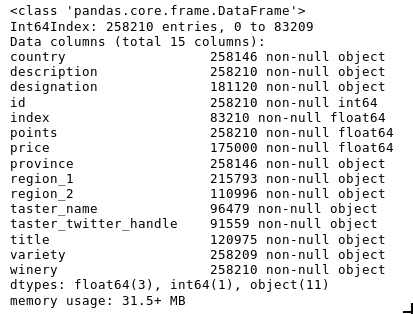
\includegraphics[width=0.59\linewidth]{infoD}	
	 \begin{itemize}
		\item We can see that the total number of columns is 15
		
		\item We can also see the number of non-null value of each columns and their type.
	\end{itemize} 
	
\end{frame}	
	
		\begin{frame}{Explanatory Data Analysis}
			\frametitle{Explanatory Data Analysis}
			
			Now let's look at the distribution of Points and Prices \\
			
			\centering
			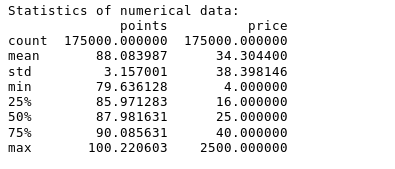
\includegraphics[width=0.65\linewidth]{statisticalNumericalD}	 \begin{itemize}
				\item The values of points are distributed between 80 and 100

				\item Mean price of 34.3 and average points is 88
				
			\end{itemize} 
		
		\end{frame}	
	
	\begin{frame}{Explanatory Data Analysis}
	\frametitle{Explanatory Data Analysis}
	\begin{figure}
	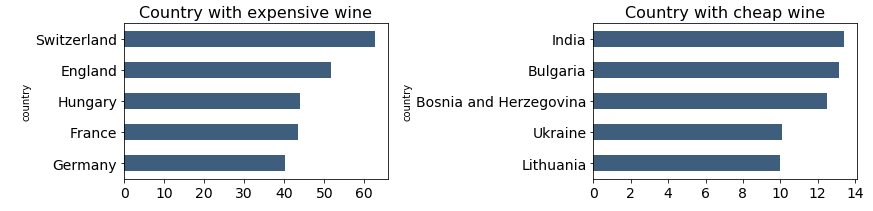
\includegraphics[width=\linewidth]{CountrybyPrice}

	\end{figure}
\begin{itemize}
	\item Most expensive wine is from Switzerland
	\item Cheapest wine is from India
\end{itemize}
	
	\end{frame}	

	
		\begin{frame}{Explanatory Data Analysis}
	\frametitle{Explanatory Data Analysis}
	\begin{figure}
		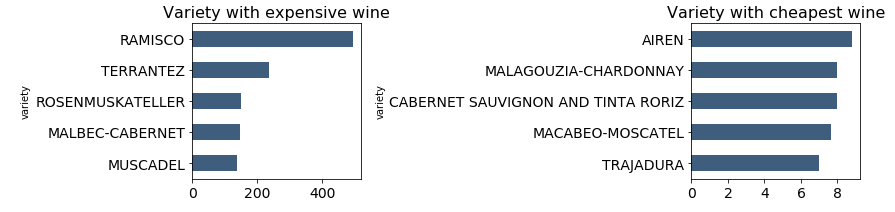
\includegraphics[width=\linewidth]{VarietybyPrice}
		
	\end{figure}
	\begin{itemize}
		\item Most expensive variety is Ramisco.
		\item Cheapest variety is Airen.
	\end{itemize}
	
\end{frame}	
\section{Feature Engineering}
\begin{frame}{Feature Engineering}
\frametitle{Feature Engineering}

\begin{figure}
	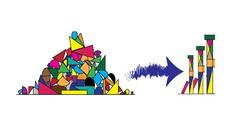
\includegraphics[width=\linewidth,height=0.4\linewidth]{featureengineering}
	
\end{figure}
\begin{itemize}
	\item Label encoding
	\item One Hot Encoding
	\item TF-IDF
\end{itemize}


\end{frame}	
	
	\section{Algorithms Used }
		\begin{frame}{Method : Random Forest Regression}
		\frametitle{Random Forest Regression}
		
		Random forest is a Supervised Learning algorithm.
		\begin{figure}
			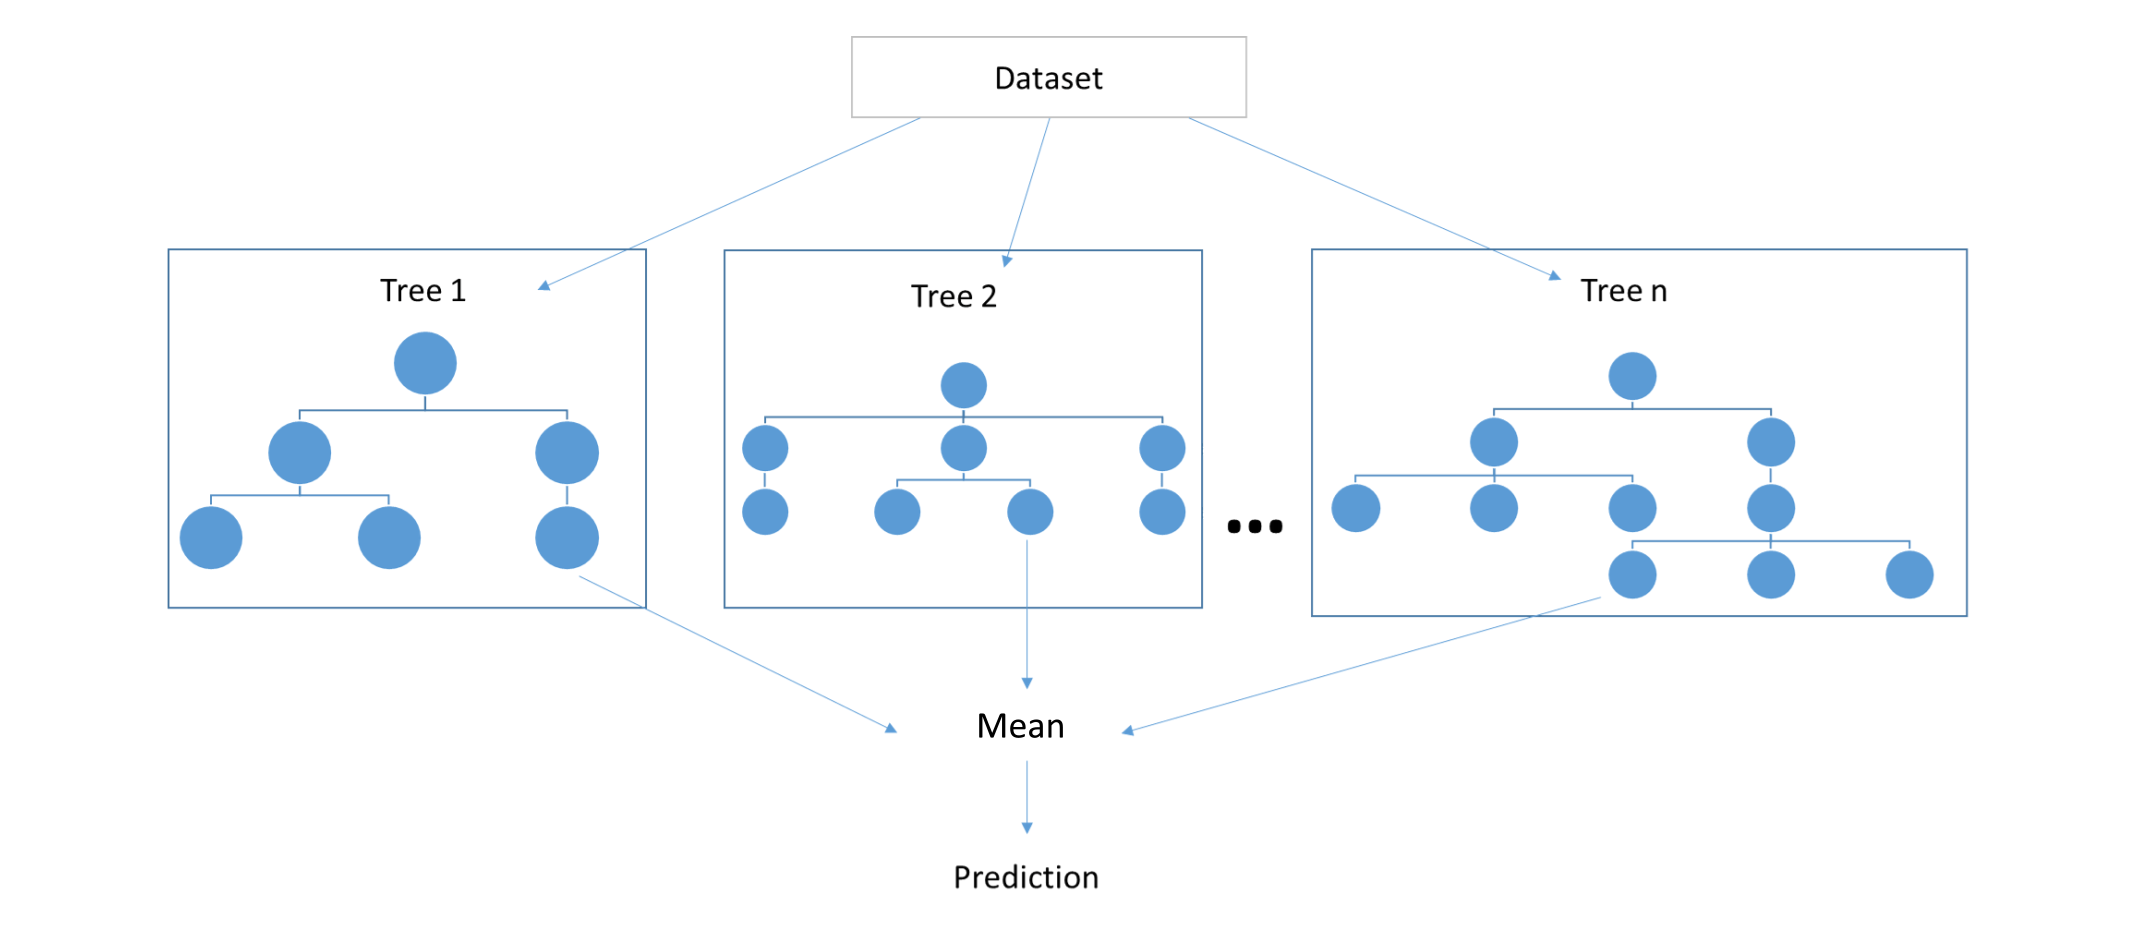
\includegraphics[width=\linewidth,height=0.5\linewidth]{Random_forest}
			
		\end{figure}
%		\begin{block}{Random Forest Intuition}
%			\begin{itemize}
%				\item \textbf{Step 1 :} Pick at K data points from the training data
%				\item \textbf{Step 2 :} Build the decision tree associated to these K data points	
%				\item \textbf{Step 3 :} Choose the number N-tree of trees you want to build and repeat \textbf{Steps 1 and 2}
%				\item \textbf{Step 4 :} For a new data point, make each one of your N-tree trees predict the value of label(Y) to for the data point in question, and assign the new data point the average across all the predicted label(Y) value.
%			\end{itemize}
%		\end{block}
%		\begin{itemize}			
	
%		\end{itemize}
		

		
	\end{frame}	

		\begin{frame}{Method :XGBoost}
	\frametitle{XGBoost}
	
\begin{itemize}
	\item Supervised machine learning algorithm
	\item Predicts target variable by combining estimates of simpler, weaker models.
	\item Incrementally building an ensemble by training each new
	model instance to emphasize the training instances that previous models mis-classified.
\end{itemize}	
	
\end{frame}	
		\begin{frame}
		\frametitle{Results}

		\begin{table}[]
			\begin{tabular}{lll}
				\hline
				\textbf{Model}          & \textbf{RMSE (Validation)} & \textbf{RMSE (Test)} \\ \hline
				Random Forest Regressor & 21.6                       &                      \\
				XGBoost Regressor       & 23.8                       &                      \\
				XGB + Random Forest     & 22.7                       & 20.43                \\ \hline
			\end{tabular}
		\end{table}
	\begin{itemize}
		\item 10-Fold cross validation applied in both models.
		\item Random Forest performs better than XGBoost.
		\item Combining the models gives even better results. 
	\end{itemize}
	\end{frame}
			
	\section{Conclusion}
	
		\begin{frame}{}
		
			\begin{block}{Conclusion}
			Two models were used with cross validation. Their predictions were averaged and RMSE of 20.4 was achieved.
			\end{block}
		\end{frame}
	
		\begin{frame}{References}
			\frametitle{References}
			\begin{itemize}
%				\item \url{https://www.slideshare.net/akhileshjoshi123/random-forest-regression?from_action=save}
				\item \url{http://webdropin.com/wordpress99/answering-wine-related-questions-with-data/}
				\item \url{https://www.udemy.com/course/feature-engineering-for-machine-learning/}
			\end{itemize}
		
		\end{frame}
	
	\begin{frame}{}
	
			\begin{flushleft}
				
\includegraphics[width=0.6\linewidth, height=0.80\textheight]{thanks}
			\end{flushleft}
	
	\end{frame}
		

%	\begin{frame}
%		\frametitle{}
%	\end{frame}

\end{document}